%Gliederung:
%
%Abstract
%Einleitung <--- Martin
%       Geschichte
%        Wozu, Verbreitungsgrad
%        Anwendungsgebiete
%Funktionsweise: Aufbau und Ablauf einer PPP-Verbindung <--- Michael Sch.
%        Header, Payload
%        (Verschiedene Arten von PPP)
%        Unterprotokolle
%Alternativen zu PPP <--- Michael St.
%        Vergleich mit anderen Protos (zB SLIP: http://comment.univie.ac.at/95-3/19/) oder DOCSIS
%                (aktuelle) Alternativen
%Schlussfolgerung
%Danksagungen (Acknowledgements)
\documentclass[journal]{IEEEtran}
\hyphenation{op-tical net-works semi-conduc-tor} 
\usepackage[pdftex]{graphicx}
\begin{document} 
\title{Das Grundprinzip von PPP - \\wie es funktioniert, pros und cons} 
\author{\IEEEauthorblockN{Martin Hellwig, Michael Schulze, Michael Stahn}
\IEEEauthorblockA{\\Kommunikationsnetze 1\\ Technische Universit\"at Darmstadt\\} }
\maketitle 
\begin{abstract} 
The abstract goes here. The abstract is abstract because it's abstrct. (qed) Was laberst du?^^
\end{abstract} 
\begin{IEEEkeywords} 
PPP, PPPoE, PPPoA, Point-to-Point. 
\end{IEEEkeywords}
\section{Einleitung} 
\IEEEPARstart{D}{as} Point-to-Point Protocol wurde urspr\"unglich im Jahr 1994 von W. Simpson entwickelt. Im OSI-Modell ist es zusammen mit anderen Protokollen in der DataLink-Schicht daf\"ur zust\"andig eine direkte Verbindung zwischen zwei Clients herzustellen. Für diesen Zweck werden auch M\"oglichkeiten der Authentifizierung spezifiziert. \cite{RFC1661} \\
Die Notwendigkeit dieses Protokolls war zu dieser Zeit sehr hoch, da \"altere Standards, wie SLIP oder ISDN, nicht mehr zeitgem\"a\ss{} waren. Speziell für die Internetverbindung für Heimanwender wurde f\"ur den alten ISDN-Standard ein Ersatz erschaffen. Mit den beiden Unter-Protokollen PPPoE (Point-to-Point over Ethernet)\cite{RFC2516} und PPPoA (Point-to-Point over ATM)\cite{RFC2364} kann man sich nun mithilfe eines Routers direkt mit dem Provider verbinden, was h\"ohere Datenraten zul\"asst. Dabei bleibt aber weiterhin der Vorteil (welcher zum Beispiel bei ISDN vorhanden ist), dass man zeitgebundene Tarife für die Endkunden anbieten kann. Bei heutigen DSL-Anschl\"ussen besitzt man zwar eine dauerhafte physikalische Verbindung zum Provider, doch erst mit dem Aufbau der PPP-Verbindung ist man auch virtuell mit dem Provider verbunden und kann somit das Internet nutzen. \\
In folgendem Bild (siehe Bild \ref{fig:PPP-Visualisierung}) wird gezeigt f\"ur welchen Zweck das PPP-Protokoll bei DSL-Zug\"angen genutzt wird. Dabei stellt der heimische Router eine feste virtuelle Verbindung zu der Gegenstelle des Providers her, welche (aktuell in Deutschland so geregelt) im Normalfall alle 24 Stunden neu aufgebaut wird, da dann die Verbindung seitens des Anbieters automatisch getrennt wird. \\
\begin{figure}[h!]
 \centering
  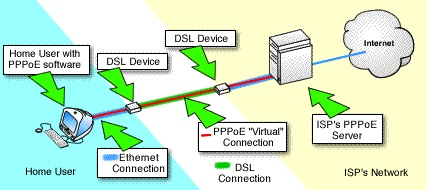
\includegraphics[width=0.5\textwidth]{gfx/PPP-Visualisierung}
 \caption{Darstellung einer PPP-Verbindung zwischen Heimanwender und ISP (Entnommen aus \cite{PPP-Bild})}
 \label{fig:PPP-Visualisierung}
\end{figure}
Neben DSL-Anschl\"ussen gibt es in Deutschland die Alternative des Kabel-Anschlusses. Bei Kabel-Anschl\"ussen wird nicht das PPP-Protokoll zum Aufbau einer Verbindung genutzt, sondern das DOCSIS-Protokoll zusammen mit einer DHCP-\"ahnlichen \cite{RFC3256} Funktionsweise. 
\section{Conclusion} 
The conclusion goes here. 
\subsection{Subsection Heading Here} 
Subsection text here. 
% needed in second column of first page if using \IEEEpubid 
%\IEEEpubidadjcol 
\subsubsection{Subsubsection Heading Here} 
Subsubsection text here. 
\appendices 
\section{Proof of the First Zonklar Equation} 
Appendix one text goes here. 
% you can choose not to have a title for an appendix 
% if you want by leaving the argument blank 
\section{} 
Appendix two text goes here. 
% use section* for acknowledgement 
\section*{Acknowledgment} 
The authors would like to thank... 
% Can use something like this to put references on a page 
% by themselves when using endfloat and the captionsoff option. 
\ifCLASSOPTIONcaptionsoff 
  \newpage 
\fi
\begin{thebibliography}{1} 
\bibitem{IEEEhowto:kopka} 
H.~Kopka and P.~W. Daly, \emph{A Guide to \LaTeX}, 3rd~ed.\hskip 1em plus 
  0.5em minus 0.4em\relax Harlow, England: Addison-Wesley, 1999. 
Andrew S. Tanenbaum: Computer Networks, 5.th edition, Prentice Hall, 2011
James F. Kurose / Keith W. Ross, Computernetzwerke, Pearson, 2012
RFC 1661 – Point-to-Point Protocol (PPP) July 1994;
RFC 1662 – Point-to-Point Protocol in HDLC-like Framing
RFC 1962, PPP Compression Control Protocol (CCP)
RFC 1963, PPP Serial Data transport Protocol
RFC 1990, The PPP Multilink Protocol (MP)
RFC 1994, PPP Challenge Handshake Authentication Protocol (CHAP)
RFC 2153, Informational, PPP Vendor Extensions
RFC 2284, PPP Extensible Authentication Protocol (EAP)
RFC 2364, PPP over ATM
RFC 2516, PPP over Ethernet
RFC 2615, PPP over SONET/SDH
RFC 2686, The Multi-Class Extension to Multi-Link PPP
RFC 2687, Proposed Standard, PPP in a Real-time Oriented HDLC-like Framing
RFC 5072, IP Version 6 over PPP
RFC 5172, Negotiation for IPv6 Datagram Compression Using IPv6 Control Protocol
RFC 6361, PPP Transparent Interconnection of Lots of Links (TRILL) Protocol Control Protocol
\bibitem{RFC2637} Point-to-Point Tunneling Protocol (IETF RFC 2637), \newblock K. Hamzeh, \newblock The Internet Society, \newblock Juli, \newblock 1999.
\bibitem{RFC1661} Point-to-Point Protocol (IETF RFC 1661), \newblock W. Simpson, \newblock The Internet Society, \newblock Juli, \newblock 1994.
\bibitem{RFC2364} Point-to-Point Protocol over AAL5 (IETF RFC 2364), \newblock  G. Gross, \newblock The Internet Society, \newblock Juli, \newblock 1998.
\bibitem{RFC2516} Point-to-Point Protocol over Ethernet (IETF RFC 2516), \newblock  L. Mamakos, \newblock The Internet Society, \newblock Februar, \newblock 1999.
\bibitem{RFC3256} The DOCSIS (Data-Over-Cable Service Interface Specifications) Device Class DHCP (Dynamic Host Configuration Protocol) Relay Agent Information Sub-option (IETF RFC 3256), \newblock  D. Jones
, \newblock The Internet Society, \newblock April, \newblock 2002.
\bibitem{PPP-Bild} Veranschaulichung einer PPP-Verbindung, \newblock  Vicomsoft
, \newblock http://www.vicomsoft.com/learning-center/pppoe/.
\end{thebibliography} 
\end{document} 
